\documentclass[a4paper, 10pt, twocolumn]{amsart}

\usepackage[nokoma,noindent,fancytheorems,fancyproofs]{adam}
\usepackage[margin=0.75in]{geometry}
\usepackage{tikz-cd}

\setlist[enumerate]{leftmargin=8mm}
\setlist[itemize]{leftmargin=8mm}

\newcommand{\enumpre}{\vspace{-1.5\baselineskip}}



% NOTE: for a more compact, black and white style for printing, use
% the below.

% \documentclass[a3paper, 10pt]{amsart}

% \usepackage[nokoma, noindent]{adam}
% \usepackage[landscape,margin=0.5in]{geometry}
% \usepackage{tikz-cd}
% \usepackage{multicol}

% \setlist[enumerate]{leftmargin=8mm}
% \setlist[itemize]{leftmargin=8mm}

% \newcommand{\enumpre}{}
% % \newcommand{\enumpre}{\vspace{-1.5\baselineskip}}
% \renewcommand{\vocab}[1]{\emph{#1}}

\newcommand{\dom}{\operatorname{dom}}
\newcommand{\card}{\operatorname{card}}
\newcommand{\on}{\operatorname{On}}

\title{Logic and Set Theory}
\author{Adam Kelly -- Mathematical Tripos Part II}
\date{\today. Email \texttt{ak2316@srcf.net}}

\begin{document}
% \begin{multicols*}{5}
\maketitle

\section{Propositional Logic}

\subsection{Languages}

We begin with \emph{propositional logic}.

\begin{definition}[Language]
  Let $P$ be a set of \vocab{primitive propositions}. Unless otherwise stated, $P = \{p_1$, $p_2, \dots\}$. The \vocab{language} $L$ or $L(P)$ is defined inductively by
  \begin{enumerate}
    \item If $p \in P$, then $p \in L$.
    \item $\bot \in L$ (where we read $\bot$ as `false')
    \item If $p, q \in L$ then $(p \Rightarrow q) \in L$.
  \end{enumerate}
\end{definition}

Every \vocab{proposition} (member of $L$) is a finite string of symbols from the alphabet $\{(,),\Rightarrow, \bot, p_1, p_2, \dots\}$, satisfying some grammar.

The precise inductive definition is as follows. Let $L_1 = P \cup \{\bot\}$, and define $L_{n + 1} = L_n \cup \{(p \Rightarrow q) \mid p, q \in L_n\}$. Then $L = \cup_{n = 1}^{\infty} L_n$.
Note there is exactly one way in which any element of the language can be constructed from the rules above.

We introduce the abbreviations $\lnot$ (not), $\land$ (and), and $\lor$ (or) defined by 
$$
\lnot p = (p \Rightarrow \bot); \quad p \land q = \lnot(p \Rightarrow \lnot q); \quad p \lor q = \lnot p \Rightarrow q.
$$

\subsection{Semantic Implication}

We now assign some sort of `true' or `false' values to propositions.

\begin{definition}[Valuation]
  A \vocab{valuation} is a function $v : L \rightarrow \{0, 1\}$ (where we think of $0$ as false and 1 as true) such that
  \begin{enumerate}
    \item $v(\bot) = 0$
    \item $v(p \Rightarrow q) = 0$ if $v(p) = 1$ and $v(q) = 0$, and $1$ otherwise.
  \end{enumerate}
\end{definition}

% \begin{remark}
%   We could put a structure on $\{0, 1\}$ where we define the constant $\bot = 0$ and define the operation $\Rightarrow$ in the obvious way. Then a valuation would be a homomorphism from $L$ to this structure on $\{0, 1\}$. 
% \end{remark}

% Valuations are determined by how they act on the primitives.
\begin{proposition}[Valuations Defined on Primitives]~
  \enumpre
  \begin{enumerate}[label=(\roman*)]
    \item Let $v, v' : L \rightarrow \{0, 1\}$ be valuations that agree on the primitives $p_i$. Then $v = v'$.
    \item Any function $w: P \rightarrow \{0, 1\}$ extends to a valuation.
  \end{enumerate}
\end{proposition}
% \begin{proposition}[Valuations Defined on Primitives]
% (i) Let $v, v' : L \rightarrow \{0, 1\}$ be valuations that agree on the primitives $p_i$. Then $v = v'$.
    
% (ii) Any function $w: P \rightarrow \{0, 1\}$ extends to a valuation.
% \end{proposition}
\begin{proof}(i) Clearly $v, v'$ agree on $L_1$. Then if they agree on $p, q$, they agree on $p \Rightarrow q$. So by induction they agree on $L_n$ for all $n$, and hence on $L$.

  (ii) Let $v(p) = w(p)$ for all $p \in P$, and $v(\bot) = 0$ to obtain $v$ on the set $L_1$. Assuming $v$ is defined on $p, q$ we can define it at $p\Rightarrow q$ in the obvious way. This defines $v$ on all of $L$.
\end{proof}

\begin{definition}[Tautology]
  A \vocab{tautology} is an element $t \in L$ such that $v(t) = 1$ for any valuation $v$. We write $\models t$.
\end{definition}

Some examples of tautologies are $p \Rightarrow (q \Rightarrow p)$ and $\lnot \lnot p \Rightarrow p$.

\begin{definition}[Semantic Implication]
  Let $S \subseteq L$ and $t \in L$. We say $S$ \vocab{entails} or \vocab{semantically implies} $t$, written $S \models t$, if $v(t) = 1$ whenever $v(s) = 1$ for all $s \in S$.
\end{definition}
\begin{definition}[Model]
  We say that $v$ is a \vocab{model} of $S$ in $L$ if $v(s) = 1$ for all $s \in S$.
\end{definition}

So the statement $S \models t$ is the statement that every model of $S$ is also a model of $t$. We also note that the notation $\models t$ is equivalent to $\emptyset \models t$.

\subsection{Syntactic Implication}

For a notion of proof, we require a system of axioms and deduction rules.

\begin{axiom}[Axiom Scheme]~
  \enumpre
  \begin{enumerate}
    \item $p \Rightarrow (q \Rightarrow p)$ for all $p, q \in L$;
    \item $[p \Rightarrow (q \Rightarrow r)] \Rightarrow [(p \Rightarrow q) \Rightarrow (p \Rightarrow r)]$ for all $p, q \in L$;
    \item $(\lnot \lnot p) \Rightarrow p$ for all $p \in L$.
  \end{enumerate}
\end{axiom}

For our deduction rules, we will only have \vocab{modus ponens}: from each $p$ and $p \Rightarrow q$ we can deduce $q$.

\begin{definition}[Syntactic Implication/Proof]
  For $S \subseteq L$, and $t \in S$ we say $S$ \vocab{proves} or \vocab{syntactically implies} $t$, written $S \vdash t$, if there exists a sequence $t_1, \dots, t_n=t$ in $L$ with every $t_i$ is either an axiom, a member of $S$ or $q$ where $t_j = p$ and $t_k = p \Rightarrow q$ and $j, k < i$.

  We say that $S$ is the set of \vocab{premises} or \vocab{hypotheses}, and $t$ is the \vocab{conclusion}.
\end{definition}

\begin{example}
  We will prove $\{p\Rightarrow q, q \Rightarrow r\} \vdash p \Rightarrow r$.

  \begin{enumerate}
    \item $q \Rightarrow r$ \hfill (Hyp)
    \item $(q \Rightarrow r) \Rightarrow(p \Rightarrow(q \Rightarrow r))$ \hfill (Ax 1)
    \item $p \Rightarrow(q \Rightarrow r)$ \hfill (MP on 2, 3)
    \item $[p \Rightarrow(q \Rightarrow r)] \Rightarrow[(p \Rightarrow q) \Rightarrow(p \Rightarrow r)]$ \hfill (Ax 2)
    \item $(p \Rightarrow q) \Rightarrow(p \Rightarrow r)$ \hfill (MP on 3, 4)
    \item $p \Rightarrow q$ \hfill (Hyp)
    \item $p \Rightarrow r$ \hfill (MP on 5, 6$)$
  \end{enumerate}
\end{example}

\begin{definition}[Theorem]
  If $\emptyset \vdash t$, we say that $t$ is a \vocab{theorem}, written $\vdash t$.
\end{definition}

\begin{example}
  We will prove the theorem $\vdash (p \Rightarrow p)$.

  \begin{enumerate}
    \item $(p \Rightarrow((p \Rightarrow p) \Rightarrow p)) \Rightarrow((p \Rightarrow(p \Rightarrow p)) \Rightarrow(p \Rightarrow p))$ \hfill(Ax 2)
    \item $p \Rightarrow((p \Rightarrow p) \Rightarrow p)$ \hfill(Ax 1)
    \item $(p \Rightarrow(p \Rightarrow p)) \Rightarrow(p \Rightarrow p)$ \hfill(MP on 1, 2)
    \item $p \Rightarrow(p \Rightarrow p)$ \hfill(Ax 1)
    \item $p \Rightarrow p$ \hfill(MP on 3, 4)
  \end{enumerate}
\end{example}

\subsection{The Deduction Theorem}

Often, showing $S \vdash p$ is made easier by the idea that provability corresponds to the connective `$\Rightarrow$' in $L$. 

\begin{theorem}[Deduction Theorem]
  Let $S \subseteq L$ and $p, q \in L$. Then $S \vdash (p \Rightarrow q)$ if and only if $S \cup \{p\} \vdash q$. 
\end{theorem}
\begin{proof}
Given a proof of $p \Rightarrow q$ from $S$, add the line $p$ by hypothesis and deduce $q$ from modus ponens, to obtain a proof of $q$ from $S \cup\{p\}$.

Conversely, suppose we have a proof of $q$ from $S \cup\{p\}$. Let $t_1, \ldots, t_n$ be the lines of the proof. We will prove that $S \vdash\left(p \Rightarrow t_i\right)$ for all $i$.
\begin{itemize}
  \item If $t_i$ is an axiom, we write $t_i$ (Ax); $t_i \Rightarrow\left(p \Rightarrow t_i\right.$) (Ax 1); $p \Rightarrow t_i$ (MP).
  \item If $t_i \in S$, we write $t_i$ (Hyp); $t_i \Rightarrow\left(p \Rightarrow t_i\right)$ (Ax 1); $p \Rightarrow t_i$ (MP).
  \item If $t_i=p$, we write the proof of $\vdash p \Rightarrow p$ given above.
  \item If $t_i$ is obtained by MP from $t_j$ and $t_k = t_j \Rightarrow t_i$, 
  assume by induction that $S \vdash p \Rightarrow t_k$ and $S \vdash p \Rightarrow\left(t_j \Rightarrow t_i\right)$. Then write $\left(p \Rightarrow\left(t_j \Rightarrow t_i\right)\right) $ $\Rightarrow\left(\left(p \Rightarrow t_j\right) \Rightarrow\left(p \Rightarrow t_i\right)\right)$ (Ax 2); $\left(p \Rightarrow t_j\right) \Rightarrow\left(p \Rightarrow t_i\right)$ (MP); $p \Rightarrow t_i$ (MP).
\end{itemize}\vspace{-1pc}
\end{proof}

\begin{example}[Using the Deduction Theorem]
  To show $\{p \Rightarrow q, q \Rightarrow r\} \vdash p \Rightarrow r$, the deduction theorem says that it's sufficient to show that $\{p, p\Rightarrow q, q \Rightarrow r\} \vdash r$, which is just modus ponens twice.
\end{example}

\subsection{The Completeness Theorem}

We want to prove that $S \models t \iff S \vdash t$, the \vocab{completeness theorem}.
This is made up of the \vocab{soundness} statement, $S \vdash t \Rightarrow S \models t$ (`our axioms and deduction rule are not silly'), and the \vocab{adequacy statement}, $S \models t \Rightarrow S \vdash t$ (`our axioms are strong enough to deduce from $S$ every semantic consequence of $S$').

\begin{proposition}[Soundness]
  Let $S \subseteq L$, $t \in L$. Then $S \vdash t$ implies that $S \models t$.
\end{proposition}
\begin{proof}
  We have a proof of $t$ from $S$. We have $v(p) = 1$ for all $p \in S$ (as $v$ is a model of $S$) and $v(p) = 1$ for every axiom $p$ (as each axiom is a tautology), and if $v(p) = 1$ and $v(p \Rightarrow q) = 1$ then $v(q) = 1$. Hence each line $t_i$ of our proof of $t$ from $S$ has $v(t_i) =1 $.
\end{proof}

% Now let's think about adequacy in the case of $t = \bot$. If our axioms are adequate, $S \models \bot$ implies $S \vdash \bot$, so $S \not \vdash \bot$. We say that $S$ is \vocab{consistent} if $S \not \vdash \bot$. Therefore, in an adequate system, if $S$ has no models then $S$ is inconsistent.
% Equivalently, if $S$ is consistent then it has a model.

% The idea that consistent axiom sets have a model actually implies adequacy in general. Indeed, if $S \models t$, then $S \cup \{\lnot t\}$ has no models, and so it is inconsistent by assumption. Then $S \cup \{\lnot t\} \vdash \bot$, so $S \vdash \not t \Rightarrow \bot$ by the deduction theorem, giving $S \vdash t$ by our third axiom.

% So we want to construct a model of $S$, given that we know that $S$ is consistent. We would like to write down $v(t) = 1$ if $t \in S$ and $0$ otherwise, but this doesn't work on the set $S = \{p_1, p_1 \Rightarrow p_2 \}$ (as it would evaluate $p_2$ to false). It seems like we have a closure issue.

\begin{definition}[Consistent]
  We say that $S$ is \vocab{consistent} if $S \not\vdash \bot$.
\end{definition}

A special case of adequacy is $S \models \bot \Rightarrow S \vdash \bot$ (or taking the contrapositive, $S$ is consistent implies $S$ has a model).

This special case implies adequacy in general. Given $S \models t$, we have that $S \cup \{\lnot t\}$ has no model, so we should know $S \cup \{\lnot t \} \vdash \bot$ hence $S \vdash ((\lnot t) \Rightarrow \bot)$ (by the deduction theorem), so $S \vdash (\lnot \lnot t)$, but axiom 3 gives $S \vdash ((\lnot \lnot t) \Rightarrow t)$ thus $S \vdash t$ by modus ponens.

\begin{definition}[Deductive Closure]
  We say a set $S \subseteq L$ is \vocab{deductively closed} if $p \in S$ whenever $S \vdash p$. Any set $S$ has a \vocab{deductive closure}, which is the (deductively closed) set of statements $\{t \in L \mid S \vdash t\}$ that $S$ proves. 
\end{definition}

% If $S$ is consistent, then the deductive closure of $S$ is also consistent. Computing the deductive closure before the valuation solves the problem for our problematic example above, but if a primary proposition $P$ is not in $S$ but $\not p$ is not in $S$, this technique still does not work (as it would assign false to both $p$ and $\lnot p$). This is our only other issue it turns out, and to fix it we try to extend $S$ by `swallowing up', for each $p$, one of $p$ and $\lnot p$.

\begin{theorem}[Model Existence Lemma]
Every consistent $S \subseteq L$ has a model.
\end{theorem}
\begin{proof}
  First we note that for any consistent $S \subseteq L$ and $p \in L$, $S \cup \{p\}$ or $S \cup \{\lnot p\}$ is consistent\footnote{If not, then $S \cup \{p\} \vdash \bot$ and $S \cup \{\lnot p\} \vdash \bot$ so $S \vdash (p \Rightarrow \bot)$, that is, $S \vdash (\lnot p)$. Hence from $S \cup \{\lnot p\} \vdash \bot$ we obtain $S \vdash \bot$.}. Since $L$ is countable, we can list it as $t_1, t_2, \dots$. 
  Let $S_0 = S$, $S_1 = S_0 \cup \{t_1\}$ or $S_0 \cup \{\lnot t_1\}$ (so that $S_1$ is consistent), and continue on. Set $\overline{S} = S_0 \cup S_1 \dots$. Then for all $t \in L$, either $t \in \overline{S}$ or $(\not t) \in \overline{S}$.

  We can easily see inductively (since proofs are finite) that $\overline{S}$ is consistent, and also that $\overline{S}$ is deductively closed (as otherwise we'd have introduced an inconsistency). So we now define $v: L \rightarrow \{0, 1\}$ by
  $$
  v(t) = \begin{cases}
        1 & t \in \overline{S}\\
        0 & \text{otherwise}
       \end{cases}.
  $$
  We then need only to check $v$ is a valuation. To see $v(\bot) = 0$, we note $\overline{S}$ consistent implies that $\bot \not \in \overline{S}$. 

  Now suppose $v(p)=1, v(q)=0$. Then $p \in \bar{S}$ and $q \notin \bar{S}$, and we want to show $(p \Rightarrow q) \notin \bar{S}$. If this were not the case, we would have $(p \Rightarrow q) \in \bar{S}$ and $p \in \bar{S}$, so $q \in \bar{S}$ as $\bar{S}$ is deductively closed.

  Now suppose $v(q)=1$, so $q \in \bar{S}$, and we need to show $(p \Rightarrow q) \in \bar{S}$. Then $\bar{S} \vdash q$, and by axiom 1, $\bar{S} \vdash q \Rightarrow(p \Rightarrow q)$. Therefore, since $\bar{S}$ is deductively closed, $(p \Rightarrow q) \in \bar{S}$.

  Finally, suppose $v(p)=0$, so $p \notin \bar{S}$. We want to show $(p \Rightarrow q) \in \bar{S}$. We know that $\neg p \in \bar{S}$, so it suffices to show that $p \Rightarrow \bot \vdash p \Rightarrow q$. By the deduction theorem, this is equivalent to proving $\{p, p \Rightarrow \bot\} \vdash q$, or equivalently, $\bot \vdash q$. But by axiom $1, \bot \Rightarrow(\neg q \Rightarrow \bot)$ where $(\neg q \Rightarrow \bot)=\neg \neg q$, so the proof is complete by axiom 3.
\end{proof}

\begin{corollary}[Adequacy]
  Let $S \subseteq L$, $t \in L$. Then $S \models t$ implies that $S \vdash t$. 
\end{corollary}

Putting our soundness and adequacy statements together, we get completeness.

\begin{theorem}[Completeness Theorem for Propositional Logic]
  Let $S \subseteq L$ and $t \in L$. Then $S \models t$ if and only if $S \vdash t$.
\end{theorem}

Directly from the completeness theorem we get a series of interesting consequences.

\begin{theorem}[Compactness Theorem]
  Let $S \subseteq L$ and $t \in L$ with $S \models t$. Then there exists a finite subset $S' \subseteq S$ such that $S' \models t$.
\end{theorem}
\begin{proof}
  This follows directly from the completeness theorem, since proofs depend on only finitely many hypotheses in $S$.
\end{proof}

\begin{corollary}[Compactness Theorem, Equivalent Form]
  Let $S \subseteq L$. Then if every finite subset $S' \subseteq S$ has a model, then $S$ has a model. 
\end{corollary}

\begin{theorem}[Decidability]
  Let $S \subseteq L$ and $t \in L$. Then there is an algorithm to decide (in finite time) if $S \vdash t$.
\end{theorem}
\begin{proof}
  Trivial by replacing $\vdash$ with $\models$, by drawing the relevant truth tables.
\end{proof}


\section{Well-Ordering and Ordinals}

\subsection{Well-Orderings}

We will now talk about orderings on sets.

\begin{definition}[Total Order]
  A \vocab{total order} is a pair $(X, <)$ where $X$ is a set and $<$ is a relation on $X$ that is
  \begin{enumerate}
    \item \emph{irreflexive}: for all $x \in X$, $x \not< x$;
    \item \emph{transitive}: for all $x, y, z \in X$, $x < y$ and $y < z$ implies $x < z$;
    \item \emph{trichotomous}: for all $x, y \in X$, either $x < y$, $y < x$ or $x = y$. 
  \end{enumerate}
\end{definition}

We can instead have defined a total order in terms of $\leq$ in the obvious way (with reflexivity, transitivity, antisymmetry and trichotomy). 

\begin{definition}[Well-Ordering]
  A total order $(X, <)$ is a \vocab{well-ordering} if every (non-empty) subset of $X$ has a least element.
%   , i.e.
%   $$
% (\forall S \subseteq X)[S \neq \emptyset \Rightarrow (\exists x) (\forall y \in S) y \geq x].
%   $$
\end{definition}


\begin{proposition}[Decreasing Sequence Condition]
  $(X, <)$ is a well-ordering if and only if there does not exist a strictly decreasing sequence in $X$.
\end{proposition}

Well-orderings allow us to perform (strong) induction on a set.

\begin{proposition}[Principle of Induction]
  Let $X$ be well-ordered and let $S \subseteq X$ be such that whenever $y \in S$ for all $y < x$ then $x \in S$. Then $S = X$.
\end{proposition}
\begin{proof}
  Suppose $S \neq X$. Then there is a least $x \in X \backslash S$. Then $y \in S$ for all $y < x$ but $x \not \in S$ which is a contradiction.
\end{proof}

We will identify total orders as isomorphic in the natural way.


\begin{definition}[Order Isomorphism]
  We say that two total orders $X$ and $Y$ are \vocab{order isomorphic} if there exists a bijection $f: X \rightarrow Y$ such that $x < y \iff f(x) < f(y)$.
\end{definition}

\begin{proposition}
  Let $X, Y$ be isomorphic well-orderings. Then there exists a unique isomorphism.
\end{proposition}
\begin{proof}
  Let $f, g: X \rightarrow Y$ be two isomorphisms. Suppose that for some $x \in X$, we have $f(y) = g(y)$ for all $y < x$. Define $S = \{f(y) \mid y < x\}$, and note $S = \{g(y) \mid y < x\}$ by assumption.
  Then $Y \backslash S$ is non-empty as $f(x) \not \in S$, so it has a least element say $a$. We must then have $f(x) = a$, and by the same logic $g(x) = f(x) = a$. So by induction $f(x) = g(x)$ for all $x \in X$.
\end{proof}

\subsection{Initial Segments}

Given an ordered set, we can remove the end of the set and keep the beginning. What we are left with is an initial segment.
% We have setup induction for well-ordered sets, now we want to setup recursion for totally ordered sets.
% \vspace{\baselineskip}

\begin{definition}[Initial Segment]
  A subset $I$ of a totally ordered set $X$ is a \vocab{initial segment} if $x \in I$ implies $y \in I$ for all $y < x$.
\end{definition}

\begin{proposition}[Initial Segments in Well-Orderings]
  Every initial segment of a well-ordered set $X$ is of the form $I_x = \{y \in X \mid y < x\}$ for some $x$.
\end{proposition}
\begin{proof}
  We can see that $I_x$ is clearly an initial segment for any $x \in X$, and if $Y$ is any initial segment, we can take $x = \min X \backslash Y$ to get $Y = I_x$.
\end{proof}

We now want to show that every subset of a well-ordering $X$ is isomorphic to an initial segment of $X$. To do this we need to build a notion of recursion.

% For example, in any total ordering $X$ and $x \in X$, the set $I_x = \{y \mid y < x\}$ is an initial segment. Not all initial segments are of this form (for example $\{x \mid x \leq 3\}$ in $\R$ or $\{x \mid x > 0, x^2 < 2\}$ in $\Q$).

% In a well-ordering, every proper initial segment is of this form, indeed $I = \{y \mid y < x\}$ where $x$ is the least element of $X \backslash I$.

% Our aim is to show that every subset of a well-ordering $X$ is isomorphic to an initial segment of $X$.

\begin{theorem}[Definition by Recursion]
Let $X$ be a well-ordering and let $Y$ be any set. Take $G: \mathcal{P}(X \times Y) \rightarrow Y$ (i.e a `rule'). Then there exists a unique function $f: X \rightarrow Y$ such that $f(x) = G\left(\left.f\right|_{I_x}\right)$ for all $x \in X$.
\end{theorem}
\begin{proof}
Say that $h$ is an `attempt' if $h : I \rightarrow Y$ for some initial segment $I$ of $X$, and for all $x \in I$ we have $h(x) = G\left(\left.h\right|_{I_x}\right)$. 

If we have two attempts $h, h'$ both defined at $x$, then they must agree, by induction on $x$.

For all $x$, there also exists an attempt defined at $x$, by induction on $x$. Indeed, by induction we can assume there exists an attempt $h_y$ defined at $y$ for all $y<x$, and then we can define $h$ to be the union of the $h_y$. This is an attempt with domain $I_x$, so the attempt $h^{\prime}=h \cup\{x, G(h)\}$ is an attempt defined at $x$. Therefore, there is an attempt defined at each $x$, so we can define the function $f: X \rightarrow Y$ by setting $f(x)$ to be the value of $h(x)$ where $h$ is some attempt defined at $x$.

For uniqueness, we apply induction on $x$. If $f, f^{\prime}$ agree below $x$, then they must agree at $x$ since $f(x)=G\left(\left.f\right|_{I_x}\right)=G\left(\left.f^{\prime}\right|_{I_x}\right)=f^{\prime}(x)$.
\end{proof}

We can now prove our result by recursively sending minimum elements of our subset to minimum elements of our set.

\begin{proposition}[Subset Collapse]
  Any subset $Y$ of a well-ordering $X$ is isomorphic to a unique initial segment of $X$.
\end{proposition}
\begin{proof}
For $f: X \rightarrow Y$ to be an order preserving bijection with an initial segment of $x$, we need to map $x$ to the smallest thing not yet mapped to, that is, $f(x) = \min(X \backslash \{f(y) \mid y < x\})$. 
We can take this minimum since $f(z)<x$ for all $z < x$, and hence $x$ is in this set. Then, by the recursion theorem, this function exists and is unique.
\end{proof}

\begin{corollary}
  A well-ordered $X$ can \emph{never} be isomorphic to a proper initial segment of itself.
\end{corollary}
\begin{proof}
  Since $X$ is isomorphic to itself by the identity function, and uniqueness shows that it cannot be isomorphic to another initial segment.
\end{proof}

\subsection{Relating Well-Orderings}

We now want to be able to talk more about the structure of well-orderings.

\begin{definition}[Comparing Well-Orderings]
  For well-orderings $X, Y$, we will write $X \leq Y$ if $X$ is isomorphic to an initial segment of $Y$.
\end{definition}

By subset collapse, $X \leq Y$ if and only if $X$ is isomorphic to some subset of $Y$.
% Note that $X \leq Y$ if and only if $X$ is isomorphic to some subset of $Y$. 

\begin{proposition}[Trichotomy]
  Let $X$, $Y$ be well-orderings. Then either $X \leq Y$, $Y \leq X$ or both (in which case $X$ and $Y$ are isomorphic). 
\end{proposition}
\begin{proof}
  Consider $f: X \rightarrow Y$ given by $f(x) = \min (Y \backslash \{f(y) \mid y < x\})$. If this is well-defined, then it is an isomorphism from $X$ to an initial segment of $Y$. If it is not well-defined, there is some $x$ such that $\{f(y) \mid y < x\} = Y$, but then $f$ is a isomorphism between $I_x$ and $Y$. Hence either $X \leq Y$ or $Y \leq X$ or both. 

If both hold, let $g: Y \rightarrow X$ be defined similarly and consider $g \circ f: X \rightarrow X$. This is an isomorphism from $X$ to an initial segment of $X$, and hence all of $X$ (as the initial segment can't be proper). For this to occur we must have that $f$ and $g$ are isomorphisms between $X$ and $Y$.
\end{proof}


\subsection{Constructing Larger Well-Orderings}

% For well-orderings $X$, $Y$, we say $X < Y$ if $X \leq Y$ and $X$ is not isomorphic to $Y$. Equivalently if and only if $X$ is isomorphic to a proper initial segment of $Y$.

Given a well-ordering, we can extend it by exactly one element.

\begin{definition}[Successor]
  Given a well-ordering $X$, choose some $x \not \in X$ and define a well-ordering on $X \cup \{x\}$ by setting $y < x$
  for all $y \in X$. This is \vocab{successor} of $X$, written $X^+$. 
\end{definition}
We clearly have $X < X^+$.
We can also `stick a bunch of well-orderings together'.

\begin{definition}[Extensions]
  Given well-orderings $(X, <_X)$ and $(Y, <_Y)$ we say $Y$ \vocab{extends} $X$ if $X$ is a proper initial segment of Y and $<_X, <_Y$ agree when both defined.

We say well-orderings $\{X_i \mid i \in I\}$ are \vocab{nested} if for all $i, j$ one of $X_i$ and $X_j$ extends the other.
\end{definition}

\begin{proposition}[Extending Well-Orderings]  
  Let $\{X_i \mid i \in I\}$ be a nested set of well-orderings. Then there exists a well-ordering $X$ such that $X_i \leq X$ for all $i$.
\end{proposition}
\begin{proof}
  Let $X = \cup_i X_i$ with the ordering given by $<_X = \cup_i <_i$. That is, $x < y$ in $X$ if there exists $i$ such that $x, y \in X_i$ and $x <_i y$.

  Given $S \subseteq X$ non-empty, we have $S \cap X_i$ non-empty for some $i\in I$. Let $x$ be the least element in this (under $<_i$). Then $x$ is the least element of $S$ in $X$ since $X_i$ is an initial segment of $X$, by nestedness. So $X$ is a well-ordering, and $X \geq X_i$ for all $i$.
\end{proof}


\subsection{Ordinals}

We will now introduce a more convenient way of talking about well-orderings.
% With what we have looked at so far, a natural question is whether the collection of al well-orderings itself form a well-ordering? To look at this, we are going to discuss the kinds of well-ordered sets that can occur by defining \emph{ordinals}.

\begin{definition}[Ordinal]
  An \vocab{ordinal} is a well-ordered set, where we regard two ordinals as equal if they are isomorphic.
\end{definition}

\begin{definition}[Order Type]
If a well-ordering $X$ has corresponding ordinal $\alpha$, we say $X$ has \vocab{order type} $\alpha$, and write $\operatorname{otp}(X) = \alpha$.
\end{definition}
  
The order type of the unique well-ordering on a collection of $k \in \N$ points is named $k$. The order type of $(\N, <)$ is named $\omega$. 

% \begin{example}[Examples of Order Types]
%   In the reals, the order type of the set $\{-2, 3, \pi, 5\}$ is 4, and the set $\{1/2, 2/3, 3/4, \dots \}$ has order type $\omega$.
% \end{example}

For ordinals $\alpha, \beta$, write $\alpha \leq \beta$ if $X \leq Y$ for some $X$ of order type $\alpha$ and $Y$ of order type $\beta$. This does not depend on the choice of $X$ and $Y$ (since any two choices must be isomorphic).

% We will also write $I_\alpha = \{\beta \mid \beta < \alpha\}$.

\begin{proposition}[$I_\alpha$ is Well-Ordered]
  For any ordinal $\alpha$, $I_\alpha = \{\beta \mid \beta < \alpha\}$ form a well-ordered set of order type $\alpha$. 
\end{proposition}
\begin{proof}
  Let $\operatorname{otp}(X) = \alpha$. 
  Then well-orderings $<X$ are precisely (up to isomorphism) the proper initial segments of $X$ (by uniqueness of subset collapse). But these are the $I_x$ for all $x \in X$, so we can biject $X$ with the well-orderings $<X$ by $x \mapsto I_x$.
\end{proof}

\begin{proposition}[The Ordinals are Well-Ordered]
  Every non-empty set $S$ of ordinals has a least element.
\end{proposition}
\begin{proof}
Choose $\alpha \in S$. If it is minimal, done. If not, then $S \cap I_\alpha$ is non-empty, but $I_\alpha$ is well-ordered and hence has a least element, $\beta$. Then this is a minimal element of $S$.
\end{proof}

However, the ordinals do not form a well-ordered \emph{set} because of the following.
% However:

\begin{theorem}[Burali-Forti Paradox]
  The ordinals do not form a set.
\end{theorem}
\begin{proof}
  Suppose $X$ was the set of all ordinals. Then since it's well-ordered it has an order type say $\alpha$. Thus $X$ is order-isomorphic to $I_\alpha$, so $X$ is order-isomorphic to a proper initial subset of itself, which is a contradiction.
\end{proof}

\begin{definition}[Supremum]
  Let $S = \{\alpha_i \mid i \in I\}$ be a set of ordinals. We define $\sup S$ to be the \vocab{supremum} or \vocab{least upper bound} of $S$.
\end{definition}

We note that the least upper bound exists since an upper bound exists (taking $\alpha$ arising from extending the nested family of well orderings $I_{\alpha_i}$), and $I_{\alpha}$ is a set.

\subsection{Examples of Ordinals}
We already know the ordinals $\{0, 1, 2, 3, \dots, \omega\}$. Writing $\alpha + 1$ for the successor $\alpha^+$ of $\alpha$, this along with the supremum allows us to generate a lot of ordinals. 

\begin{center}
  \small
  \begin{tabular}{ccccccc}
    0 & $\omega\cdot 2 + 1$ & $\omega^2 + 1$ & $\omega^2\cdot 3$ & $\omega^{\omega + 2}$ & $\varepsilon_0 + 1$ \\
    1 & $\omega\cdot 2 + 2$ & $\omega^2 + 2$ & $\omega^2\cdot 4$ & $\vdots$ & $\vdots$ \\
    2 & $\omega\cdot 2 + 3$ & $\omega^2 + 3$ & $\omega^2\cdot 5$ & $\omega^{\omega \cdot 2}$ & $\varepsilon_0 \cdot 2$ \\
    $\vdots$ & $\vdots$ & $\vdots$ & $\vdots$ & $\vdots$ & $\vdots$ \\
    $\omega$ & $\omega\cdot 3$ & $\omega^2 + \omega$ & $\omega^3$ & $\omega^{\omega^2}$ & $\varepsilon_0^2$ \\
    $\omega + 1$ & $\omega\cdot 4$ & $\vdots$ & $\vdots$ & $\vdots$ & $\vdots$ \\
    $\omega + 2$ & $\omega\cdot 5$ & $\omega^2 + \omega \cdot 2$ & $\omega^\omega$ & $\omega^{\omega^{\omega}}$ & $\varepsilon_0^{\varepsilon_0}$ \\
    $\vdots$ & $\vdots$ & $\vdots$ & $\vdots$ & $\vdots$ & $\vdots$ \\
    $\omega + \omega$ & $\omega\cdot \omega $ & $\omega^2 \cdot 2$ & $\omega^{\omega + 1}$ & $\omega^{\omega^{.^{.^.}}}$ & $\varepsilon_0^{\varepsilon_0^{.^{.^.}}}$ \\
    $=\omega\cdot 2$ & $=\omega^2$ & &  & $= \varepsilon_0$ & $= \varepsilon_1$ \\
  \end{tabular}
\end{center}

We have used some new notation, for example $\omega + 1 = \omega^+$ and $\omega \cdot 2 = \sup \{\omega, \omega+1, \cdots$. We will formally define this later.

Each of the ordinals above are countable, as at each step we are only adding one element and taking countable unions. This question is equivalent to asking can we well order $\R$, and we find that we can though we can't write it down.

\begin{theorem}[Uncountable Ordinal Existence]
  There is an uncountable ordinal.
\end{theorem}
\begin{proof}
  % We want to take the supremum of the set of countable ordinals, so we check that that is a set.
  Let $A = \{R \in \mathcal{P}(\omega \times \omega) \mid$ $R$ is a well ordering of a subset of $\omega \}$. 
  Then $B = \{\operatorname{otp}(R) \mid R \in A\}$ is the set of all countable ordinals. 

  Let $\omega_1 = \sup B$. If $\omega_1$ was countable, it would be in $B$. But then $\omega_1 < \omega_1^+ \in B$ is a contradiction, so $\omega_1$ is uncountable.


  Alternatively we could say that $B$ isn't all ordinals since they don't form a set (Burali-Forti), forcing there to be an uncountable ordinal. 
\end{proof}
We note $\omega_1$ is the \emph{least} uncountable ordinal by the definition of $B$.

The ordering $\omega_1$ has some remarkable properties. For example all of the proper initial segments of $\omega_1$ are countable but $\omega_1$ is not. Also any sequence $\alpha_1, \alpha_2, \dots$ in $I_{\omega_1}$ is bounded, namely by $\sup\{\alpha_1, \alpha_2, \dots\}$ which is countable as a countable union of countable sets.

The same argument allows us to find ordinals that don't inject into any given set.
\begin{theorem}[Hartogs' Lemma]
  For every set $X$, there exists an ordinal $\alpha$ that does not inject into $X$. We call the least such ordinal $\gamma(X)$ (read `\vocab{Hartogs' of $X$}')
\end{theorem}

So $\gamma(\omega) = \omega_1$.


\subsection{Limits and Successors}
In general we can divide ordinals into two categories.

\begin{definition}[Limits and Successors]
  We say $\alpha$ is a \vocab{successor} if there exists $\beta$ such that $\alpha = \beta^+$. Otherwise we say that $\alpha$ is a \vocab{limit}.
\end{definition}

An $\alpha$ has a greatest element if and only if it is a successor. So $\alpha$ is a limit if and only if it has no greatest element. We typically denote limit ordinals by $\lambda$. 

\subsection{Ordinal Arithmetic}

We will now make formal sense out of our arithmetic notation such as $\omega + \omega$ used earlier.

\begin{definition}[Ordinal Addition -- Inductive]
We define $\alpha + \beta$ by recursion on $\beta$ (keeping $\alpha$ fixed).
We take
\begin{align*}
  \alpha + 0 &= \alpha,\\
  \alpha + \beta^+ &= (\alpha + \beta)^+,\\
  \alpha + \lambda &= \sup\{\alpha + \gamma \mid \gamma < \lambda\},
\end{align*}
for non-zero limit $\lambda$.
\end{definition}

\begin{proposition}[Non-Commutative Addition]
  Ordinal addition is not commutative\footnote{Arises from asymmetry in decision to recurse on the right}. In particular, $\omega + 1 \neq 1 + \omega$.
\end{proposition}
\begin{proof}
  We have $\omega+1 = \omega + 0^+ = \omega^+$, and $1 + \omega = \sup\{1 + n \mid n \leq \omega\} = \sup \{1, 2, 3, \dots\} = \omega$.
\end{proof}

\begin{proposition}[Associative Addition]
  For all ordinals $\alpha, \beta, \gamma$, we have $\alpha + (\beta + \gamma) = (\alpha + \beta) + \gamma$.
\end{proposition}
\begin{proof}
We induct on $\gamma$, keeping $\alpha, \beta$ fixed. If $\gamma=0$, then $\alpha+(\beta+0)= \alpha+\beta=(\alpha+\beta)+0$.

If $\gamma = \delta^+$ is a successor, then
\begin{align*}
  \alpha + (\beta + \delta^+) &= \alpha + (\beta + \delta)^+ \\
  &= [\alpha + (\beta + \delta)]^+ = [(\alpha + \beta) + \delta]^+ \\
  &= (\alpha + \beta) + \delta^+,
\end{align*}
as required.

If $\lambda$ is a non-zero limit ordinal, we have
\begin{align*}
(\alpha+\beta)+\lambda & =\sup \{(\alpha+\beta)+\gamma: \gamma<\lambda\} \\
& =\sup \{\alpha+(\beta+\gamma): \gamma<\lambda\} .
\end{align*}
We claim that $\beta+\lambda$ is a limit.
Indeed, we have $\beta+\lambda=\sup \{\beta+\gamma: \gamma<\lambda\}$. 
But $\lambda$ is a limit, so for every $\gamma < \lambda$, we can find a $\gamma'$ with $\gamma < \gamma' < \lambda$. So $\beta + \gamma' > \beta + \gamma$, so $\beta + \gamma$ cannot be the greatest element.

Now $\alpha + (\beta + \lambda) = \sup\{\alpha + \delta \mid \delta < \beta + \lambda\}$.
We need to show that 
$$\sup\{\alpha + \delta \mid \delta < \beta +\lambda\} = \sup \{\alpha + (\beta + \gamma) \mid \gamma < \lambda\}.
$$
Now each element on the right is an element of the left, so we get that the left is $\geq$ the right. Also, for $\delta < \beta + \lambda$ we have $\delta < \sup \{\beta + \gamma \mid \gamma < \lambda\}$, so $\delta < \beta + \gamma$ for some $\gamma < \lambda$. Hence $\alpha + \delta < \alpha + (\beta + \gamma)$. Thus the left is $\leq$ the right too, and thus these supremums must be equal.
\end{proof}

We can give an alternative definition of addition based on actual well-orders, intuitively by writing all of the elements of $\alpha$ followed by all the elements of $\beta$.
\[
  \alpha + \beta = \underbrace{\quad\quad\vphantom{\beta}\alpha\vphantom{\beta}\quad\quad}\underbrace{\quad\;\beta\;\quad}
\]
\begin{definition}[Ordinal Addition -- Synthetic]
  $\alpha + \beta$ is the order type of $\alpha \sqcup \beta$ with all $\alpha$ before all of $\beta$.
\end{definition}

\begin{proposition}[Addition Notion Equivalence]
  The inductive and synthetic definitions of addition coincide.
\end{proposition}
\begin{proof}
We write $+$ for the inductively defined one, and $+'$ for the synthetic one. We'll show $\alpha + \beta = \alpha +' \beta$ for all $\alpha + \beta$ by induction on $\beta$ (with $\alpha$ fixed). We check the cases
\begin{enumerate}
  \item \emph{zero}: $\alpha + 0 = \alpha = \alpha +' 0$;
  \item \emph{successor}: $\alpha + \beta^+ = (\alpha + \beta)^+ = (\alpha +' \beta)^+$, which is the order type of 
  $$
  \underbrace{\quad\quad\vphantom{\beta}\alpha\vphantom{\beta}\quad\quad}\underbrace{\quad\;\beta\;\quad}
  \underbrace{\vphantom{\beta}\bullet\vphantom{\beta}}
  $$ 
  which is $\alpha +' \beta^+$.
  \item \emph{non-zero limit}: $\alpha + \lambda = \sup\{\alpha + \gamma \mid \gamma < \lambda\} = \sup\{\alpha +' \gamma \mid \gamma < \lambda\} = \alpha +' \lambda$ (since the supremum is a union as sets are nested).
\end{enumerate}\vspace{-1pc}
\end{proof}

We can then define multiplication, both inductively and synthetically.

\begin{definition}[Ordinal Multiplication -- Inductive]
  We define $\alpha \cdot \beta$ by recursion on $\beta$ (keeping $\alpha$ fixed). We take
  \begin{align*}
    \alpha \cdot 0 &= 0, \\
    \alpha \cdot (\beta^+) &= \alpha \cdot \beta + \alpha, \\
    \alpha \cdot \lambda = \sup \{\alpha \cdot \gamma \mid \gamma < \lambda\},
  \end{align*} 
  for non-zero limit $\lambda$.
\end{definition}

Diagrammatically, our synthetic definition is given by
$$
\alpha \cdot \beta = \underbrace{
  \underbrace{\alpha}
  \underbrace{\alpha}
  \cdots
  \underbrace{\alpha}
}_{\beta\text{ times}}.
$$

\begin{definition}[Ordinal Multiplication -- Synthetic]
  $\alpha \cdot \beta$ is the order type of $\alpha \times \beta$, with $(x, y) < (x', y')$ if $y < y'$ or ($y = y'$ and $x < x'$).
\end{definition}

We can again check that the inductive and synthetic definition agree, that ordinal multiplication is again not commutative ($\omega \cdot 2 = \omega + \omega$ but $2 \cdot \omega = \omega$) but that it is associative and so on in the exact same way as we did for addition.

We can also define exponentiation. We will give only the inductive definition.

\begin{definition}[Ordinal Exponentiation]
  We define $\alpha^\beta$ by induction on $\beta$. We take
  \begin{align*}
    \alpha^0 &= 1, \\
    \alpha^{\beta^+} &= \alpha^\beta \cdot \alpha, \\
    \alpha^\lambda &= \sup \{\alpha^\gamma \mid \gamma < \lambda\},
  \end{align*}
  where $\lambda$ is a non-zero limit ordinal.
\end{definition}


\section{Posets and Zorn's Lemma}

\subsection{Posets and Hasse Diagrams}

We now look at posets and eventually arrive at a statement and proof of Zorn's lemma.

\begin{definition}[Poset]
  A \vocab{partially ordered set} or \vocab{poset} is a pair $(X, \leq)$, where $X$ is a set and $\leq$ is a relation on $X$ that is reflexive, transitive and antisymmetric (if $x \leq y$ and $y \leq x$ then $x = y$). We write $x < y$ if $x \leq y$ and $x \neq y$. In terms of $<$, a poset is irreflexive and transitive.
\end{definition}

\begin{example}[Examples of Posets]~
  \enumpre
  \begin{enumerate}
    \item Any total order.
    \item $(\N^+, `\text{divides}')$
    \item For $S$ any set, take $\mathcal{P}(S)$ with $A \leq B$ if $A \subset B$.
    \item Take $X$ to be any subset of $\mathcal{P}(S)$ with the same $\leq$.
    \item Consider
    % q=WzAsNSxbMiwyLCJhIl0sWzEsMSwiYiJdLFswLDAsImMiXSxbMywxLCJkIl0sWzQsMCwiZSJdLFswLDEsIiIsMCx7InN0eWxlIjp7ImhlYWQiOnsibmFtZSI6Im5vbmUifX19XSxbMSwyLCIiLDAseyJzdHlsZSI6eyJoZWFkIjp7Im5hbWUiOiJub25lIn19fV0sWzAsMywiIiwyLHsic3R5bGUiOnsiaGVhZCI6eyJuYW1lIjoibm9uZSJ9fX1dLFszLDQsIiIsMix7InN0eWxlIjp7ImhlYWQiOnsibmFtZSI6Im5vbmUifX19XV0=
\[\begin{tikzcd}[sep=tiny]
	c &&&& e \\
	& b && d \\
	&& a
	\arrow[no head, from=3-3, to=2-2]
	\arrow[no head, from=2-2, to=1-1]
	\arrow[no head, from=3-3, to=2-4]
	\arrow[no head, from=2-4, to=1-5]
\end{tikzcd}\]
meaning $a \leq b$, $b \leq c$, $a \leq d$, $d \leq e$ and everything following from transitivity. So $a \leq c$ but $b$ and $d$ are unrelated.
  \end{enumerate}
\end{example}

\begin{definition}[Hasse Diagram]
  A \vocab{Hasse diagram} of a poset consists of a drawing of the points in $X$ with an upward line from $x$ to $y$ if $y$ \vocab{covers} $x$ (meaning $y > x$ and no $z$ has $y > z > x$).
\end{definition}

\begin{example}[Examples of Hasse Diagrams]~
  \enumpre
  \begin{enumerate}
    \item % https://q.uiver.app/?q=WzAsNSxbMSwzLCJhIl0sWzAsMSwiYiJdLFsxLDAsImMiXSxbMiwyLCJkIl0sWzIsMSwiZSJdLFswLDEsIiIsMCx7InN0eWxlIjp7ImhlYWQiOnsibmFtZSI6Im5vbmUifX19XSxbMSwyLCIiLDAseyJzdHlsZSI6eyJoZWFkIjp7Im5hbWUiOiJub25lIn19fV0sWzAsMywiIiwyLHsic3R5bGUiOnsiaGVhZCI6eyJuYW1lIjoibm9uZSJ9fX1dLFszLDQsIiIsMix7InN0eWxlIjp7ImhlYWQiOnsibmFtZSI6Im5vbmUifX19XSxbNCwyLCIiLDIseyJzdHlsZSI6eyJoZWFkIjp7Im5hbWUiOiJub25lIn19fV1d
    \[\begin{tikzcd}[sep=tiny]
      & c \\
      b && e \\
      && d \\
      & a
      \arrow[no head, from=4-2, to=2-1]
      \arrow[no head, from=2-1, to=1-2]
      \arrow[no head, from=4-2, to=3-3]
      \arrow[no head, from=3-3, to=2-3]
      \arrow[no head, from=2-3, to=1-2]
    \end{tikzcd}\]
    (so we have no notion of `height' or `rank')
  \item % https://q.uiver.app/?q=WzAsNSxbMCwyLCJhIl0sWzIsMiwiYiJdLFsyLDEsImQiXSxbMCwxLCJjIl0sWzEsMCwiZSJdLFswLDIsIiIsMix7InN0eWxlIjp7ImhlYWQiOnsibmFtZSI6Im5vbmUifX19XSxbMCwzLCIiLDAseyJzdHlsZSI6eyJoZWFkIjp7Im5hbWUiOiJub25lIn19fV0sWzMsNCwiIiwwLHsic3R5bGUiOnsiaGVhZCI6eyJuYW1lIjoibm9uZSJ9fX1dLFsyLDQsIiIsMix7InN0eWxlIjp7ImhlYWQiOnsibmFtZSI6Im5vbmUifX19XSxbMSwyLCIiLDIseyJzdHlsZSI6eyJoZWFkIjp7Im5hbWUiOiJub25lIn19fV0sWzEsMywiIiwyLHsic3R5bGUiOnsiaGVhZCI6eyJuYW1lIjoibm9uZSJ9fX1dXQ==
  \[\begin{tikzcd}[sep=tiny]
    & e \\
    c && d \\
    a && b
    \arrow[no head, from=3-1, to=2-3]
    \arrow[no head, from=3-1, to=2-1]
    \arrow[no head, from=2-1, to=1-2]
    \arrow[no head, from=2-3, to=1-2]
    \arrow[no head, from=3-3, to=2-3]
    \arrow[no head, from=3-3, to=2-1]
  \end{tikzcd}\]
  \end{enumerate}
\end{example}

\begin{definition}[Chain]
  A subset $S$ of a poset $X$ is a \vocab{chain} if it is a total order. 
  We say $S$ is an \vocab{antichain} if no two members of $S$ are related by order.
\end{definition}

% \begin{example}[Examples of Chains/Antichains]
%   In a total order, every subset is a chain.
%   In the poset $(\N^+, `\text{divides}')$, $\{1, 2, 4, 8, \dots\}$ is a chain, and $\{p \mid p\text{ prime}\}$ is an antichain.
% \end{example}

\begin{definition}[Supremum]
  For $S \subset X$, we say $x \in X$ is an \vocab{upper bound} for $S$ if $y \leq x$ for all $y \in S$. We say $x$ is a \vocab{least upper bound} or \vocab{supremum} for $S$ if $x$ is an upper bound for $S$, and every upper bound $y$ for $S$ has $y \geq x$. We write $\sup S = x$.
\end{definition}

\begin{definition}[Complete]
  A poset $X$ is \vocab{complete} if every set $S \subset X$ has a supremum.
\end{definition}

In any complete poset $X$, there is a greatest element ($\sup X$), and a least element $(\sup \emptyset)$.

\begin{definition}[Order Preserving Map]
  For a poset $X$, a function $f: X \rightarrow X$ is \vocab{order-preserving} if $x \leq y$ implies $f(x) \leq f(y)$.
\end{definition}

\begin{theorem}[Knaster-Tarski Fixed Point Theorem]
  Let $X$ be a complete poset, and $f: X \rightarrow X$ order-preserving. Then $f$ has a fixed point.
\end{theorem}
\begin{proof}
  Let $E = \{x \in X \mid x \leq f(x)\}$, and let $s = \sup E$. We claim $f(s) =s$.

  To show $s \leq f(s)$, enough to show that $f(s)$ an upper bound for $E$ (then $s \leq f(s)$ as $s$ is the least upper bound). But $x \in E \Rightarrow x \leq s \Rightarrow f(x) \leq f(s) \Rightarrow x \leq f(x) \leq f(s)$.

To show $f(s) \leq s$, enough to show that $f(s) \in E$ (as $s$ is an upper bound for $E$). But $s \leq f(s)$, so $f(s) \leq f(f(s))$ (as $f$ order-preserving), i.e. $f(s) \in E$.
\end{proof}

\begin{corollary}[Schr\"oder-Bernstein Theorem]
  Let $A, B$ be sets, and let $f: A \rightarrow B$ and $g: B \rightarrow A$ be injections. Then there exists a bijection from $A$ to $B$.
\end{corollary}
\begin{proof}
  We try to partition $A$ into $P$ and $Q$, and $B$ into $R$ and $S$, such that $f(P) = R$ and $g(S) = Q$. Then we let $h = f$ on $R$ and $g^{-1}$ on $Q$.
  \begin{center}
    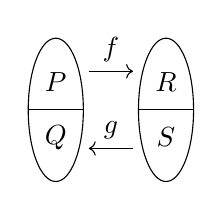
\begin{tikzpicture}[scale=0.7]
      \draw (-1, 0) ellipse (0.5 and 1.3);
      \draw (-1.5, 0) -- (-0.5, 0);
      \node at (-1, -0.5) {$Q$};
      \node at (-1, 0.5) {$P$};
      \draw (1, 0) ellipse (0.5 and 1.3);
      \draw (0.5, 0) -- (1.5, 0);
      \node at (1, -0.5) {$S$};
      \node at (1, 0.5) {$R$};
      \draw [->] (-0.4, 0.7) -- (0.4, 0.7) node [pos = 0.5, above] {$f$};
      \draw [->] (0.4, -0.7) -- (-0.4, -0.7) node [pos = 0.5, above] {$g$};
    \end{tikzpicture}
  \end{center}
  Since $S = B\setminus R$ and $Q = A \setminus P$, so we want
  \[
    P = A\setminus g(B\setminus f(P))
  \]
  Since the function $P \mapsto A\setminus g(B\setminus f(P))$ from $\mathcal{P}(A)$ to $\mathcal{P}(A)$ is order-preserving (and $\mathcal{P}(a)$ is complete), the result follows.
\end{proof}

\subsection{Zorn's Lemma}
Now we can get to the heart of the matter.

\begin{definition}[Maximal Element]
  In a poset $X$, an element $x \in X$ is \vocab{maximal}\footnote{Take care to note the difference between \emph{maximum} and \emph{maximal} elements} if no $y \in X$ has $y > x$.
\end{definition}

\begin{theorem}[Zorn's Lemma]
Assuming the Axiom of Choice, let $X$ be a (non-empty) poset in which every chain has an upper bound. Then $X$ has a maximal element.
\end{theorem}
\begin{proof}
  Suppose $X$ has no maximal element. So for each $x \in X$ there is $x' \in X$ with $x' > x$. We know that every chain $C$ has some upper bound $u(C)$. 

  Let $\gamma = \gamma(X)$ (as guaranteed by Hartog's Lemma). Pick some $x \in X$, and define $x_\alpha$, $\alpha < \gamma$ recursively by
  \begin{align*}
    x_0 &= x \\ x_{\alpha^+} &= x'_{\alpha} \\
    x_{\lambda} &= u(\{x_\alpha \mid \alpha < \lambda\}),
  \end{align*}
  for $\lambda$ a non-zero limit. Note that $\{x_\alpha \mid \alpha < \lambda\}$ is a chain, by induction. Then the $x_\alpha$, $\alpha < \gamma$, are distinct, so we have injected $\gamma$ into $X$, which is a contradiction.
\end{proof}

\subsection{Applications of Zorn}
We can use Zorn's lemma to prove some powerful results.

\begin{theorem}
  Every vector space $V$ has a basis.
\end{theorem}
\begin{proof}
  Let $X$ be the set of all linearly independent subsets of $V$, ordered by inclusion.
  We want to find a maximal element $A \in X$. If one exists, we are done as if it didn't span we could add an element not in the span and remain linearly independent, which would contradict maximality.

  We use Zorn's lemma. Given a chain $\left\{A_i: i \in I\right\}$, let $A=\cup_{i \in I} A_i$. Then $A \supset A_i$ for all $i$, so just need to check $A \in X$, that is, $A$ is linearly independent.

Suppose we have a linear dependence in $A$, say $\lambda_1 x_1+\ldots+\lambda_n x_n=0$, where $x_1, \ldots, x_n \in A$ and $\lambda_1, \ldots, \lambda_n$ are scalars (not all 0). 
We must then have $x_i \in A_{k_i}$ for $k_i \in I$, but then some $A_{k_i}$ contains all of these (as the $A_i$ are a chain), contradicting $A_{k_i}$ being linearly independent.
\end{proof}

We can also use Zorn to dispense with our assumption that our set of primitive propositions was countable in our discussion of propositional logic.

\begin{theorem}[Model Existence Lemma -- Uncountable Case]  Let $S \subset L(P)$, for any set of primitive propositions $P$. Then $S$ consistent implies $S$ has a model.
\end{theorem}
\begin{proof}
  
  We need a consistent $\bar S \subseteq S$ such that $\forall t\in L$, $t\in \bar S$ or $\neg t\in \bar S$. Then we have a valuation $v(t) = \ii[t \in \bar S]$ as in our original proof for the countable case.

  So we seek a \emph{maximal} consistent $\bar S\supseteq S$. If $\bar S$ is maximal, then if $t\not\in \bar S$, then we must have $\bar S \cup \{t\}$ inconsistent, i.e.\ $\bar S \cup \{t\}\vdash \bot$. By deduction theorem, this means that $\bar S \vdash \neg t$. By maximality, we must have $\neg t \in \bar S$. So either $t$ or $\neg t$ is in $\bar S$.

  Now we show that there is such a maximal $\bar S$. Let $X = \{ T\subseteq L: T\text{ is consistent }, T\supseteq S\}$. Then $X\not=\emptyset$ since $S\in X$. We show that any non-empty chain has an upper bound. An obvious choice is, again the union.

  Let $\{T_i: i\in I\}$ be a non-empty chain. Let $T = \bigcup T_i$. Then $T\supseteq T_i$ for all $i$. So to show that $T$ is an upper bound, we have to show $T\in X$.

  Certainly, $T\supseteq S$, as any $T_i$ contains $S$ (and the chain is non-empty). So we want to show $T$ is consistent. Suppose $T\vdash \bot$. So we have $t_1, \cdots, t_n \in T$ with $\{t_1, \cdots, t_n\} \vdash \bot$, since proofs are finite. Then some $T_k$ contains all $t_i$ since $T_i$ are nested. So $T_k$ is inconsistent. This is a contradiction. Therefore $T$ must be consistent.

  Hence by Zorn's lemma, there is a maximal element of $X$.
\end{proof}

\subsection{Zorn's Lemma and the Axiom of Choice}

We first look at one other consequence of Zorn's lemma.

\begin{theorem}[Well-Ordering Principle]
  Assuming Zorn's Lemma, Every set $S$ can be well-ordered.
\end{theorem}
\begin{proof}
  Let $X$ be the set of pairs $(A, R)$ where $A \subseteq S$ and $R$ is a well ordering of $A$, and order $X$ by $(A, R) \leq (A', R')$ if the latter extends the former. $X$ is non empty, as say $(\emptyset, \emptyset) \in X$. Now given a chain $\{(A_i, R_i) \mid i \in I\}$, we have an upper bound $\{\cup_{i \in I} A_i, \cup_{i \in I} R_i)$, since our family is nested.
So by Zorn's lemma, there exists a maximal element $(A, R)$. We must have $A = S$, as if not we can take $x \in S \backslash A$ and `take the successor': well order $A \cup \{x\}$ by making $x > y$ for all $y \in A$ which would then contradict the maximality of $(A, R)$.
\end{proof}

Now, we assumed the Axiom of Choice in our proof of Zorn's lemma, and we assumed Zorn's lemma in our proof of the Well-Ordering Principle. We will now see the Well-Ordering Principle implies the Axiom of Choice, and that all three are equivalent.

\begin{theorem}[Axiom of Choice]
  Assuming the Well-Ordering Principle, 
  If $\{A_i \mid i \in I\}$ is a family of non-empty sets, there is a \vocab{choice function} $f: I \rightarrow \cup_{i \in I} A_i$ such that $f(i) \in A_i$.
\end{theorem}
\begin{proof}
  Given our family, well-order $\cup_{i \in I} A_i$. Then we can define $f(i)$ to be the least element of $A_i$ for each $i \in I$.
\end{proof}


\section{Predicate Logic}

\subsection{Language}

We now look at a more complicated version of the style of logic that we looked at before.

\begin{definition}[Language]
  Let $\Omega$ (\vocab{function symbols}) and $\Pi$ (\vocab{relation symbols}) be disjoint sets and $\alpha: \Omega \cup \Pi \rightarrow \N$ a function (\vocab{arity}).

  The \vocab{Language} $L = L(\Omega, \Pi, \alpha)$ is the set of formulae, defined as follows:
  \begin{itemize}
    \item \emph{Variables}. We have some variables $x_1, x_2, \dots$ (also written $x, y, z, \dots$)
    \item \emph{Terms}. These are defined inductively by
    \begin{enumerate}
      \item Every variable is a term;
      \item If $f \in \Omega$, $\alpha(f) = n$ and $t_1, \dots, t_n$ are terms, then $f(t_1, \dots, t_n)$ is a term.
    \end{enumerate}
    \item \emph{Atomic formulae}. There are three sorts:
    \begin{enumerate}
      \item $\bot$;
      \item $(s = t)$ for any terms $s, t$;
      \item $\phi(t_1, \dots, t_n)$ for any $\phi \in \Pi$ with $\alpha(\phi) = n$ and $t_1, \dots, t_n$ terms.
    \end{enumerate}
    \item \emph{Formulae}. These are defined inductively by
    \begin{enumerate}
      \item Atomic formulae are formulae;
      \item $(p \Rightarrow q)$ is a formula for any formulae $p, q$;
      \item $(\forall x) p$ is a formula for any formula $p$ and variable $x$.
    \end{enumerate}
  \end{itemize}
\end{definition}

\begin{example}[The Language of Groups]
  We will give a prototypical example, the language of Groups. In this case, we have $\Omega = \{m , i, e\}$, $\Pi = \emptyset$ and $\alpha(m) = 2$, $\alpha(i) = 1$ and $\alpha(e) = 0$. Then $e, x_1, m(x_1, x_2), i(m(x_1, x_1))$ are terms and $m(e, e) = e$, $(\forall x)m(x, i(x)) = e$ are formulae.
\end{example}

Note that a formula is just a string of meaningless symbols. It doesn't make sense to ask if it's true or false. In particular the function and relation symbols are not assigned any meaning aside from its arity. 

We have the usual abbreviations as before, and we also have $(\exists x) p$ for $\lnot (\forall x)(\lnot p)$.

\begin{definition}[Closed Term]
  A term is \vocab{closed} if it has no variables.
\end{definition}

\begin{definition}[Free and Bound Variables]
  An occurrence of a variable $x$ in a formula $p$ is \vocab{bound} if it is inside brackets of a $(\forall x)$ quantifier. It is \vocab{free} otherwise.
\end{definition}

\begin{definition}[Sentence]
  A \vocab{sentence} is a formula with no free variables.
\end{definition}

\begin{definition}[Substitution]
  For a formula $p$, a variable $x$ and a term $t$, the \vocab{substitution} $p[t/x]$ is obtained by replacing each free occurrence of $x$ with $t$.
\end{definition}

\subsection{Semantic Entailment}

In propositional logic we had `valuations'. We are going to replace these with sets that have operations of the right arity, called a \emph{structure}. 

\begin{definition}[Structure]
  An \vocab{$L$-struture} is a non-empty set $A$ with a function $f_A: A^n \rightarrow A$ for each $f \in \Omega$, with $\alpha(f) = n$ and a relation $\phi_A \subseteq A^n$, for each $\phi \in \Pi, \alpha(\phi) = n$.
\end{definition}

\begin{remark}
  To make life easier, we explicitly forbid $A$ from being empty. 
\end{remark}

We now want to define\footnote{After it's defined, we can pretty much forget about it.} `$p$ holds in $A$' for a sentence $p \in L$ and an $L$-structure $A$.

\begin{definition}[Interpretation]
  To define the \vocab{interpretation} $p_A \in \{0, 1\}$ for each sentence $p$ and $L$-structure $A$, we define inductively:
  \begin{itemize}
    \item \emph{Closed terms}. Define $t_A \in A$ for each closed term $t$ by
    $$
    (f(t_1, \dots, t_n))_A = f_aA(t_{1_A}, \dots, t_{n_A}) 
    $$
    for any $f \in \Omega$, $\alpha(f) = n$ and closed terms $t_1, \dots, t_n$.
    \item \emph{Atomic formulae}. We take
    \begin{align*}
      \bot_A &=0,\\
      (s = t)_A &= \ii[s_A = t_A],\\
      (\phi(t_1, \dots, t_n))_A &= \ii[(t_{1_A}, \dots, t_{n_A}) \in \phi_A]
    \end{align*}
    \item \emph{Sentences}. We take
    \begin{align*}
      (p \Rightarrow q)_A &= \ii[\lnot(p_A = 1, q_A = 0)] \\
      ((\forall x)p)_A &= \ii[p[\overline{a}/x]_{\overline{A}}\text{ for all }a\in A]
    \end{align*}
    where for any $a \in A$, we define a new language $L'$ be adding a constant $\overline{a}$ and make $A$ into a $L'$ structure $\overline{A}$ by setting $\overline{a}_{\overline{A}} = a$.
  \end{itemize}
\end{definition}

We can now define models and entailment.

\begin{definition}[Theory]
  A \vocab{theory} is a set of sentences.
\end{definition}

\begin{definition}[Model]
  If a sentence $p$ has $p_A = 1$, we say that $p$ \vocab{holds} in $A$, or $p$ is \vocab{true} in $A$, or $A$ is a \vocab{model} of $p$. For a theory $S$, a model of $S$ is a structure that is a model for each $s \in S$.
\end{definition}

\begin{definition}[Semantic Entailment]
  For a theory $S$ and a sentence $t$, $S$ \vocab{entails} $t$, written $S \models t$, if every model of $S$ is also a model of $t$.
\end{definition}

\begin{definition}[Tautology]
  $t$ is a \vocab{tautology}, written $\models t$, if $\emptyset \models t$.
\end{definition}

Predicate logic is also called `first-order logic', where first-order means we are ranging over \emph{elements} of the structure, and not subsets.

\subsection{Syntactic Implication}

As before, we need axioms and deduction rules.

\begin{definition}[Axioms of Predicate Logic]~
  \enumpre
  \begin{enumerate}
    \item $p \Rightarrow (q \Rightarrow p)$ for any formulae $p, q $;
    \item $[p \Rightarrow (q \Rightarrow r)] \Rightarrow [(p \Rightarrow q) \Rightarrow (p \Rightarrow r)]$ for any formulae $p, q$;
    \item $(\lnot \lnot p) \Rightarrow p$ for any formula $p$.
    \item $(\forall x)(x = x)$ for any variable $x$.
    \item $(\forall x)(\forall y)((x = y) \Rightarrow (p \Rightarrow p[y/x]))$ for any variable $x, y$ and formula $p$, with $y$ not occurring bound in $p$.
    \item $[(\forall x)p] \Rightarrow p[t/x]$ for any formula $p$, variable $x$, term $t$ with no free variable of $t$ occurring bound in$p$.
    \item $[(\forall x)(p\Rightarrow q)] \Rightarrow [p\Rightarrow(\forall x)q]$ for any formulae $p$, $q$ with variable $x$ not occurring free in $p$.
  \end{enumerate}
  % The \vocab{axioms of predicate logic} consists of the 3 usual axioms, 2 to explain how `$=$' works, and 2 to explain how $\forall$ works. 
\end{definition}

\begin{definition}[Deduction Rules of Predicate Logic]
  The \vocab{deduction rules} are 
  \begin{enumerate}
    \item \emph{Modus ponens}: From $p$ and $p \Rightarrow q$, we can deduce $q$.
    \item \emph{Generalization}: From $r$, we can deduce $(\forall x)r$ provided that no premise used in the proof so far had $x$ as a free variable.
  \end{enumerate}
\end{definition}

\begin{definition}[Proof]
  A \vocab{proof} of $p$ from $S$ is a sequence of statements, in which each statement is either an axiom, a statement in $S$, or obtained via modus ponens or generalization.
\end{definition}

\begin{definition}[Syntactic Implication]
  If there exists a proof of a formula $p$ from a set of formulae $S$, we write $S \vdash p$, and say `$S$ \vocab{proves} $t$'.
\end{definition}

\begin{definition}[Theorem]
  If $S \lvert p$, we say $p$ is a \vocab{theorem} of $S$.  
\end{definition}

Now we prove the theorems we had for propositional logic.

\begin{proposition}[Deduction Theorem]
  Let $S \subseteq L$ and $p, q \in L$. Then $S \cup \{p\} \vdash q$ if and only if $S \vdash p \Rightarrow q$.
\end{proposition}
\begin{proof}
  The proof is exactly the same as the one for propositional logic, expect in the $\Rightarrow$ case, we have to check Gen. Suppose we have the lines $r$ and $(\forall x) r$ (Gen), and we have a proof of $S\vdash p \Rightarrow r$ (by induction). We want to seek a proof of $p \Rightarrow (\forall x) r$ from $S$.

  We know that no premise used in the proof of $r$ from $S \cup \{p\}$ had $x$ as a free variable, as required by the conditions of the use of Gen. Hence no premise used in the proof of $p\Rightarrow r$ from $S$ has $x$ as a free variable. Hence $S \vdash (\forall x)(p\Rightarrow r)$. If $x$ is not free in $p$, then we get $S \vdash p \Rightarrow (\forall x)r$ by Axiom 7 (and MP). If $x$ is free in $p$, then we did not use premise $p$ in our proof $r$ from $S \cup \{p\}$. So $S \vdash r$, and hence $S \vdash (\forall x) r$ by Gen. So $S \vdash p \Rightarrow (\forall x) r$.
\end{proof}


We also have the following whose proofs we omit.

\begin{proposition}[Soundness Theorem]
  Let $S$ be a set of sentences, $p$ a sentence. Then $S \vdash p$ implies $S \models p$.
\end{proposition}
\begin{theorem}[Model Existence Lemma]
  Let $S$ be a consistent set of sentences. Then $S$ has a model.
\end{theorem}

\begin{corollary}[Adequacy Theorem]
  Let $S$ be a theory, and $p$ a sentence. Then $S \models p$ implies $S \vdash p$.
\end{corollary}

\begin{corollary}[Compactness Theorem]
  Let $S$ be a theory such that every finite subset of $S$ has a model. Then so does $S$.
\end{corollary}
\begin{proof}
  Trivial if we replace `has a model' with `is consistent', because proofs are finite.
\end{proof}

We can look at some applications of this: can we axiomatize the theory of finite groups (in the language of groups)?

\begin{corollary}
  The theory of finite groups cannot be axiomatized (in the language of groups).
\end{corollary}
\begin{proof}
  Suppose theory $T$ has models all finite groups and nothing else. Let $T'$ be $T$ together with 
  \begin{align*}
    &(\exists x_1) (\exists x_2) (x_1 \neq x) \\
    &(\exists x_1)(\exists x_2)(\exists x_3)(x_1 \neq x_2 \neq x_3)\\
    &\quad\quad\vdots 
  \end{align*}
  then $T'$ has no model, sine each model has to be simultaneously arbitrarily large and finite, but every finite subset of $T'$ does have a model (say $\Z_n$ for some $n$), which is a contradiction.
\end{proof}

So `finiteness is not a first-order property'.

\begin{corollary}
  Let $S$ be a theory with arbitrarily large models.
  Then $S$ has an infinite model.
\end{corollary}
\begin{proof}
  Same as above.
\end{proof}

\begin{corollary}[Upward L\"owenheim-Skolem Theorem]
  Let $S$ be a theory with an infinite model. Then $S$ has an uncountable model.
\end{corollary}
\begin{proof}
  Add constants $\{c_i \mid i \in I\}$ to $L$ for some uncountable $I$.
  Let $T = S \cup \{\text{`}c_i \neq c_j\text{'} \mid i, j \in I, i \neq j\}$.
  Then any finite $T' \subseteq T$ has a model, since it can only mention finitely many of the $C_i$. So any infinite model of $S$ will do. Hence by compactness, $T$ has a model.
\end{proof}

\begin{theorem}[Downward L\"owenhein-Skolem Theorem]
  Let $L$ be a countable language (i.e. $\Omega$ and $\Pi$ are countable).
  Then if $S$ has a model, then it has a countable model.
\end{theorem}
\begin{proof}
  The model constructed in the proof of model existence theorem is countable.
\end{proof}


\section{Set Theory}

\subsection{Axioms of Set Theory}

We now formulate set theory as first-order theory.

\begin{definition}[Zermelo-Fraenkel Set Theory]
  \vocab{Zermelo-Fraenkel set theory} (ZF) has language $\Omega = \emptyset$, $\Pi = \{\in \}$, with arity 2.
\end{definition}

The `universe of sets' wil mean a model with these axioms, a pair $(V, \varepsilon)$, where $V$ is a set and $\in$ is a binary relation on $V$ in which the axioms are true. 

\begin{axiom}[Axiom of Extension]
  `Sets with the same members are equal':
  $$
  (\forall x)(\forall y)[(\forall z)(z \in x \Leftrightarrow z \in y) \Rightarrow x= y].
  $$
\end{axiom}

\begin{axiom}[Axiom of Separation]
`For a set $x$ and a property $p$, we can form $\{z \in x \mid p(z)\}$':
$$
(\forall t_1)\cdots (\forall t_n) (\forall x)(\exists y)(\forall z)(z \in y \Leftrightarrow z \in x \land p)
$$
for each formula $p$ with free variables\footnote{We do need parameters to say form $\{z \in x \mid z \in t\}$ for some variable $t$.} $t_1, \dots, t_n, z$.
\end{axiom}

\begin{axiom}[Axiom of Empty Sets]
  `There is an empty set':
  $$
  (\exists x) (\forall y)[\lnot y \in x].
  $$
  We write $\emptyset$ for the (unique by extension) set guaranteed by this axiom.
\end{axiom}

\begin{axiom}[Axiom of Pair Sets]
  `We can form $\{x, y\}$':
  $$
(\forall x)(\forall y)(\exists z)(\forall t)(t \in z \Leftrightarrow t = x \lor t = y).
  $$
  We write $\{x, y\}$ for this $z$, and $\{x\}$ for $\{x, x\}$.
\end{axiom}

We can now pin down what functions are.

\begin{definition}[Ordered Pair]
  The \vocab{ordered pair} $(x, y) = \{\{x\}, \{x, y\}\}$. Clearly we have $(x, y) = (z, t)$ if and only if $x = z$ and $y = t$.
  We say $x$ is an ordered pair of $(\exists y)(\exists z)(x = (y, z))$.
\end{definition}
\begin{definition}[Function]
  We say $f$ is a \vocab{function} if
  \begin{align*}
  (\forall x)(x \in f \Rightarrow x\text{ is an ordered pair})\\
  \land (\forall x)(\forall y)(\forall z) [((x, y) \in f\land (x, z) \in f) \Rightarrow y = z].
  \end{align*}
\end{definition}
\begin{definition}[Domain]
  Call $x$ the \vocab{domain} of $f$, written $x = \operatorname{dom}(f)$ if $(f \text{ is a function})\land (\forall y)(y \in x \Leftrightarrow (\exists z)((y, z) \in f))$. 
  
  Then $f: x \rightarrow y$ means $(f\text{ is a function}) \land (x = \operatorname{dom}(f)) \land (\forall z)(\forall t)((z, t) \in f \Rightarrow t \in y)$.
\end{definition}


Back to axioms.

\begin{axiom}[Axiom of Union]
  `We can form unions':
  $$
(\forall x)(\exists y)(\forall z)(z \in y \Leftrightarrow (\exists t)(t \in x \land z \in t)).
  $$
  Note that in this definition, we think of $A \cup B \cup C$ as $\bigcup \{A, B, C\}$.
\end{axiom}

\begin{axiom}[Axiom of Power Sets]
  `We can form power sets':
  $$
  (\forall x)(\exists y)(\forall z)(z \in y \Leftrightarrow z \subseteq x),
  $$
  where $z \subseteq x$ means $(\forall t)(t \in z \Leftrightarrow t \in x)$. We write $\mathcal{P}(x)$ for the set generated above.
\end{axiom}

\begin{axiom}[Axiom of Infinity]
`There is an infinite set':
$$
(\exists x)(\emptyset \in x \land (\forall y)(y \in x \Rightarrow y^+ \in x)),
$$
where $y^+ = y \cup \{y\}$. Any set that satisfies the above axiom is a successor set.
\end{axiom}

The intersection of successor sets is a successor set, so by taking the intersection of all successor sets we get a least successor set. Call this $\omega$. Then in particular if $x \subseteq \omega$ is a successor set, then $x = \omega$.

We can use this to get induction in $V$:
\begin{align*}
(\forall x)[(x \subseteq \omega \land \emptyset \in x\land
 (\forall y)(y \in x \Rightarrow y^+ \in x))\\
 \Rightarrow x= \omega].
\end{align*}


Can now define `$x$ is finite' for $(\exists y)(y \in \omega \land x$ bijects with $y)$ and `$x$ is countable' for $(x$ is finite $) \lor(x$ bijects with $\omega)$.

\begin{axiom}[Axiom of Foundation]
  `Every (non-empty) set has an $\in$-minimal element':
  $$
  (\forall x)(x \neq \emptyset \Rightarrow(\exists y)(y \in x \land(\forall z)(z \in x \Rightarrow z \notin y))) .
  $$
\end{axiom}

\subsection{Digression on Classes}

Now we want to be able to say something like `for each $x \in I$, we have some $A_i$. Now take $\{A_i \mid i \in I\}$. We would like our result to be a set, but we don't know that this thing is a function yet. We try to define `things that look like a function'.

\begin{definition}[Class]
  Let $(V, \in)$ be an $L$-structure. A \vocab{class} is a collection $C$ of points in $V$ such that, for some formula $p$ with free variable $x$ (and maybe more parameters), we have $x \in C \Leftrightarrow p$ holds. 
\end{definition}
Intuitively, everything of the form $\{x \in V \mid p(x)\}$ is a class.

\begin{definition}[Proper Class]
  We say $C$ is a \vocab{proper class} if $C$ is not a set (in $V$), that is,
  $$
\lnot (\exists y)(\forall x)(x \in y \Leftrightarrow p).
  $$
\end{definition}
\begin{definition}
  A \vocab{function-class} $F$ is a collection of ordered pairs such that there is a formula $p$ with free variables $x, y$ (and maybe more) such that
  \begin{align*}
(x, y) \in F \Leftrightarrow p\text{ holds},\\ \text{and }(x, y) \in F \land (x, z) \in F \Rightarrow y = z.
  \end{align*}
\end{definition}

\subsection{Back to Axioms}

We can now give our last axiom.

\begin{axiom}[Axiom of Replacement]
  `The image of a set under a function-class is a set'. This is an axiom scheme,
  with an instance for each first-order formula $p$:
  {\small
  \begin{align*}
      & \underbrace{\left(\forall t_1\right) \ldots\left(\forall t_n\right)}_{\text {parameters }}[\underbrace{(\forall x)(\forall y)(\forall z)(p \land p[z / y] \Rightarrow y=z)}_{p \text { is a function class }} \\
      & \Rightarrow (\forall x) \underbrace{(\exists y)(\forall z)(z \in y \Leftrightarrow(\exists t)(t \in x \land p[t / x , z / y]))}_{y \text { is image of } x}]
  \end{align*}
  }
\end{axiom}

That is all of axioms in ZF. We didn't include the Axiom of Choice though.

\begin{definition}[ZFC]
  \vocab{ZFC} is the axioms ZF + AC, where AC is the axiom of choice, `every family of non-empty sets has a choice function':
  {\small\begin{align*}
    (\forall f)[(\forall x)(x \in \operatorname{dom} f \Rightarrow f(x) \neq \emptyset) \Rightarrow \\
    (\exists g)(\operatorname{dom} g = \operatorname{dom} f) \land (\forall x)(x \in \operatorname{dom}g \Rightarrow g(x) \in f(x))].
  \end{align*}}
\end{definition}

Here we define a family of sets $\{A_i \mid i \in I\}$ to be a function $f: I \rightarrow V$ such that $i \mapsto A_i$.

\subsection{Properties of ZF}
Now we want to know what $V$ looks like.

\begin{definition}[Transitive Set]
  A set $x$ is \vocab{transitive} if every member of a member of $x$ is a member of $x$:
  $$
  (\forall y)((\exists x)(y \in z \land z \in x) \Rightarrow y \in x).
  $$
\end{definition}

\begin{lemma}
  Every $x$ is contained in a transitive set.
\end{lemma}
\begin{proof}
  We will form the set
  $$
  x \cup \left(\bigcup x\right)\cup \left(\bigcup \bigcup x\right)\cup \left(\bigcup\bigcup\bigcup x\right)\cup \cdots,
  $$
  as it will be clearly transitive and contains $x$. By the union axiom, it suffices to obtain the set $\{x,$ $\bigcup x, \bigcup \bigcup x, \dots\}$. We can get this from the axiom of replacement, which we will apply to $\omega$ with the function-class $0 \mapsto x$, $1 \mapsto \bigcup x$, $\dots$. So we just need to show that this is indeed a function-class.

  Define $f$ as an \emph{attempt} to mean
  \begin{align*}
    (f \text{ is a function}) \land (\dom f \in \omega) \land (\dom f \neq \emptyset) \\
    \land  (f(x) = 0) \land (\forall n)([(n \in \dom f) \land (n \neq 0)] \\
    \Rightarrow f(n) = \bigcup f(n - 1)).
  \end{align*}
  We can check by usual $\omega$-induction that
  \begin{align*}
    (\forall f)(\forall g)(\forall n)([(f \text{ an attempt}) \land (g \text{ an attempt}) \\ 
    \land (n \in \dom f) \land (n \in \dom g)] \Rightarrow f(n) = g(n)),
  \end{align*}
  and also that
  \begin{align*}
    (\forall n)(n \in \omega \Rightarrow (\exists f)[\\
    (f \text{ an attempt}) \land (n \in \dom f)]),
  \end{align*}
  also by $\omega$-induction using the constructions we had before. So we indeed have a function class which we can take as $p(y, z)$ where
  $
p(y, z) = (\exists f)((f$ an attempt $\land (y \in \dom f) \land (f(y) = z)).
  $
\end{proof}
\begin{remark}
  Officially, this says `let $(V, \in)$ be a model of ZF. Then [statement]. Equivalently, ZF $\vdash$ [statement] (by the completeness theorem).' Also from this proof, we know that in particular $x$ is contained in the \vocab{transitive closure} of $x$, the intersection of all transitive sets containing $x$, written $\operatorname{TC}(x)$ (as the intersection of transitive sets is transitive).
\end{remark}

We want the axiom of foundation to capture that `sets are built out of simpler sets'. With this, we should want: if $p(x)$ holds whenever $(\forall y \in x) p(y)$, then $p(x)$ holds for all $x$.

\begin{theorem}[Principle of $\in$-Induction]
  For each formula $p$ with free variables $t_1, \dots, t_n, x$:
  \begin{align*}
  \left(\forall t_1\right) \ldots\left(\forall t_n\right)[(\forall x)((\forall y)(y \in x \Rightarrow p(y)) \\
  \Rightarrow p(x)) \Rightarrow(\forall x)(p(x))]
  \end{align*}
\end{theorem}
\begin{proof}
  Given $t_1, \dots, t_n$, suppose $\lnot (\forall x)p(x)$. Then we have $\lnot p(x)$ for some $x$.

  Note that we would like to say: choose $\in$-minimal $x$ with $\lnot p(x)$, by foundation, and hence we have a contradiction. But $\{x \mid \lnot p(x)\}$ need not be a set.

  Instead, we take $t = \operatorname{TC}(\{x\})$, and $u = \{y \in t\mid \lnot p(y)\}$. Then $u \neq \emptyset$, so $u$ has a $\in$-minimal member, say $y$. Then $\lnot p(y)$, but $z \in y \Rightarrow z \in t$ by transitivity, so $z \not \in u$, that is, $(\forall z \in y)p(z)$ which is a contradiction.
\end{proof}

\begin{theorem}
  The axiom of foundation and the principle of $\in$-induction are equivalent (in the presence of the other ZF axioms).
\end{theorem}
\begin{proof}
  We already wrote down a proof of the principle of $\in$-induction from foundation, now we prove foundation. Indeed, say that $x$ is \emph{regular} to mean $(\forall y)(x \in y \Rightarrow y$ has a minimal member$)$. So foundation says every $x$ is regular. To prove this by $\in$-induction, it is enough to show that if every $y \in x$ is regular then $x$ is regular. 

  For $z$ with $x \in z$, if $x$ is minimal in $z$ we are done. Otherwise, we have a $y\in x$ such that $y \in z$. So $z$ has a minimal element (as $y$ is regular).
\end{proof}

Now we also want to do recursion, so we can define $f(x)$ in terms of the $f(y)$, $y \in x$.

\begin{theorem}[$\in$-Recursion Theorem]
Let $G$ be a function-class $((x, y) \in G \Leftrightarrow p(x, y)$ for some formula $p)$, everywhere defined.

Then there is a function-class $F$, $((x, y) \in F \Leftrightarrow q(x, y)$, some formula $q)$, everywhere defined, such that $(\forall x)(F(x) = G(\left.F\right|_x))$. Moreover, $F$ is unique.
\end{theorem}
\begin{proof}
  For existence, we say `$f$ is an attempt' if
  \begin{align*}
    (f\text{ is a function}) \land (\dom f\text{ is transitive}) \\
    \land (\forall x)(x \in \dom f \Rightarrow f(x) = G(\left.f\right|_x)),
  \end{align*}
  where this makes sense as $\dom x$ is transitive.
  Then $(\forall x)(\forall f)(\forall f')([(f, f'\text{ attempts}) \land (x \in \dom f) \land (x \in \dom f')]\Rightarrow f(x) = f'(x))$, by $\in$-induction (as if $f$ and $f'$ agree at all $y \in x$ then they agree at $x$).

  Also, $(\forall x)(\exists f)((f \text{ is an attempt}) \land (x \in \dom f))$, again by $\in$-induction.

  If each $y \in x$ has an attempt defined at $y$, then for each $y \in x$ there is a unique attempt $f_y$ defined on $\operatorname{TC}(\{y\})$. Put $f = \bigcup\{f_y \mid y \in x\}$ and put $f' = f \cup \{(x, G(\left.f\right|_x))\}$.

  So define $F$ by: $q(x, y) = `(\exists f)((f\text{ an attept}) \land (x \in \dom f) \land (f(x) = y))'$.
  
  For uniqueness, if we have suitable function-classes $F, F'$ then $(\forall x)(F(x) = F'(x))$, by $\in$-induction.
\end{proof}

\begin{remark}
  We note that $\left.F\right|_x = \{(t, F(t)) \mid t \in x\}$ \emph{is} a set, by replacement.
\end{remark}

Notice that the proofs of $\in$-induction and $\in$-recursion look similar to induction and recursion on a well-ordered set. This may inspire a thought of what properties of the `relation' $\in$, that is, the formula $p(x, y) = `x \in y'$ have we used? 

\begin{enumerate}
  \item $p$ is \vocab{well-founded} -- every non-empty set has a $p$-minimal member.
  \item $p$ is \vocab{local} -- for each $y$, $\{x \mid p(x, y)\}$ is a set, so that we can build the transitive closure.
\end{enumerate}
So for any $p(x, y)$ that is well-founded and local, we can prove $p$-induction and $p$-recursion. If $r$ is a relation on a \emph{set} $a$, then trivially $r$ is local, so to have these we only need $r$ well-founded. The theorems about well-orderings were a special case of this.

We have almost replicated all of our results about well-orderings, except for subset collapse. We will consider this now. The following definition is motivated by `can we model a given relation on a set by $\in$'?

\begin{definition}[Extensional]
  We say a relation $r$ on a set $a$ is \vocab{extensional} if
  $$
  (\forall x, y \in a)([(\forall z \in a)(z\; r\; x \Leftrightarrow z\;r\;y) \Rightarrow x = y]),
  $$
  i.e. it obeys the axiom of extension.
\end{definition}

\begin{theorem}[Mostowski Collapse Theorem]
  Let $r$ be a relation on a set $a$ that is well-founded and extensional. Then there exists a transitive set $b$, and a bijection $f: a \rightarrow b$ such that $(\forall x, y \in a)(x\; r\; y \Leftrightarrow f(x) \in f(y))$. Moreover, $b$ and $f$ are unique.
\end{theorem}
\begin{proof}
  Define $f(x) = \{f(y) \mid y\; r\; x\}$, a definition by $r$-recursion on $a$. Note that $f$ is a function by replacement (it is an image of $a$). Let $b = \{f(x) \mid x \in a\}$, which is a set by replacement.

  Then $b$ is transitive (by the definition of $f$), and $f$ surjective (by the definition of $b$), so we need to just check that $f$ is injective (then we also have $f(x) \in f(y) \Leftrightarrow x\;r\;y$). We shall show that $(\forall y \in a)(f(x) = f(y) \Rightarrow x = y)$ for each $x \in a$, by $r$-induction on $x$.

  So suppose $f(x) = f(y)$, and that $(\forall t\;r\;x)(\forall y \in a)(f(t) = f(y) \Rightarrow t = u)$. 
  We have $\{f(t) \mid t\;r\;x\} = \{f(u) \mid u\;r\;y\}$ (by the definition of $f$), so $\{t \mid t\;r\;x\} = \{u \mid u\;r\;y\}$ by our induction hypothesis, so $x = y$ by extensionality.

  For uniqueness, if $f, f'$ are suitable then $f(x) = f'(x)$ for all $x \in a$ by $r$-induction.
\end{proof}

Now we previously defined ordinals as kind of the `equivalence class' of all well-orderings, but this was a problem since the ordinals wouldn't be sets. We define them formally as follows:

\begin{definition}[Ordinal]
  An \vocab{ordinal} is a transitive set, totally ordered by $\in$.
\end{definition}

This is automatically well-ordered by $\in$, by foundation. Note then that $\emptyset, \{\emptyset\}, \{\emptyset,\{\emptyset\}\}$ are all ordinals, any $n \in \omega$ as $n = \{0, 1, \dots, n - 1\}$ as well as $\omega$ itself is an ordinal.
  
So by Mostowski, a well-ordering is order-isomorphic to a unique ordinal, and we call that ordinal the \vocab{order-type} of this well-ordering. So well orderings $x$ and $y$ are order-isomorphic if and only if they have teh same order type.

\subsection{Picture of the Universe}

We now want to see what $V$ looks like.

\begin{definition}[Von Neumann Hierarchy]
  Define sets $V_\alpha$ for $\alpha \in \on$ (the class of ordinals) by $\in$-recursion:
  \begin{align*}
    V_0 &= \emptyset, \\
    V_{\alpha^+} &= \mathcal{P}(V_\alpha), \\
    V_\lambda &= \bigcup \{V_\gamma \mid \gamma < \lambda\},
  \end{align*}
  for $\lambda$ a non-zero limit ordinal.
\end{definition}

\begin{center}
  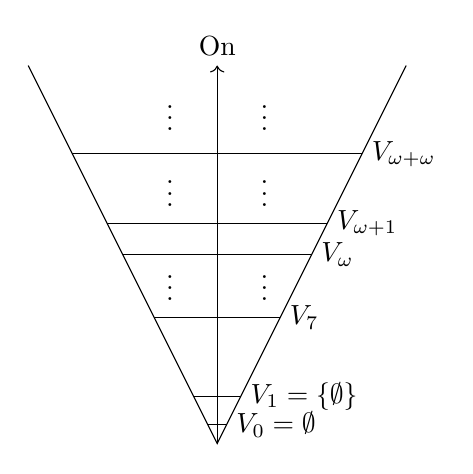
\begin{tikzpicture}[scale=0.8]
    \draw [->] (0, 0) -- (0, 6) node [above] {On};
    \draw (-3, 6) -- (0, 0) -- (3, 6);
    \draw (-0.15, 0.3) -- (0.15, 0.3) node [right] {$V_0 = \emptyset$};
    \draw (-0.375, 0.75) -- (0.375, 0.75) node [right] {$V_1 = \{\emptyset\}$};
    \draw (-1, 2) -- (1, 2) node [right] {$V_7$};
    \node at (-0.75, 2.6) {$\vdots$};
    \node at (0.75, 2.6) {$\vdots$};
    \draw (-1.5, 3) -- (1.5, 3) node [right] {$V_\omega$};
    \draw (-1.75, 3.5) -- (1.75, 3.5) node [right] {$V_{\omega + 1}$};
    \node at (-0.75, 4.1) {$\vdots$};
    \node at (0.75, 4.1) {$\vdots$};
    \draw (-2.3, 4.6) -- (2.3, 4.6) node [right] {$V_{\omega + \omega}$};
    \node at (-0.75, 5.3) {$\vdots$};
    \node at (0.75, 5.3) {$\vdots$};
  \end{tikzpicture}
\end{center}

Note that $x \subseteq V_{\alpha} \Leftrightarrow x \in V_{\alpha+1}$. We would like every $x$ to be in some $V_\alpha$, and that is indeed true.

\begin{lemma}
  Each $V_\alpha$ is transitive. 
\end{lemma}
\begin{proof}
  We induct on $\alpha$. We have $V_0$ transitive. If $V_\alpha$ is transitive then $\mathcal{P}(V_\alpha)$ is transitive, as if $x \in y \in \mathcal{P}(V_\alpha)$, then $y \subset V_\alpha$, so $x \in V_\alpha$, so $x \subset V_\alpha$ (as $V_\alpha$ transitive), so $x \in \mathcal{P}(V_\alpha)$. Finally, the union of transitive sets is transitive finishes our last case of limit ordinals.
\end{proof}

\begin{lemma}
  If $\alpha \leq \beta$, then $V_\alpha \subseteq V_\beta$.
\end{lemma}
\begin{proof}
  Fix $\alpha$ and induct on $\beta$. If $\beta = \alpha$, we are done. Given $V_\alpha \subset V_\beta$, we have $V_\beta \subset \mathcal{P}(V_\beta)$ (as $x \in V_\beta$ implies $x \subset V_\beta$, as $V_\beta$ is transitive), so $V_\alpha \subset \mathcal{P}(V_\beta) = V_{\beta^+}$. And for limits this is trivial by definition.
\end{proof}

\begin{theorem}
  Every $x$ belongs to some $V_\alpha$.
\end{theorem}
We first need to note that $x \subset V_\alpha \Leftrightarrow x \in V_{\alpha+1}$, and if $x \subset V_{\alpha}$ then there is a least such $\alpha$ called the \vocab{rank} of $x$.
\begin{proof}
  We'll show that $(\forall x)(\exists \alpha)\left(x \in V_\alpha\right)$ by $\in$-induction on $x$.

  So we are allowed to assume that for each $y \in x$, we have $y \subseteq V_\alpha$ for some $\alpha$.

  So $y \subseteq V_{\operatorname{rank}(y)}$, or $y \in V_{\operatorname{rank}(y)+1}$.
  Let $\alpha=\sup \left\{\left(\operatorname{rank}(y)^{+}: y \in x\right\}\right.$. Then $y \in V_\alpha$ for every $y \in x$. So $x \subseteq V_\alpha$   
\end{proof}

We will take the official definition of rank to be
\begin{definition}[Rank]
  The \vocab{rank} of a set $x$ is defined recursively by
  $$
\operatorname{rank}(x) = \sup \{(\operatorname{rank} y)^+ \mid y \in x\}.
  $$
\end{definition}

\begin{proposition}
  $\operatorname{rank}(x)$ is the first $\alpha$ such that $x \subseteq V_\alpha$.
\end{proposition}

\section{Cardinals}

\subsection{Basic Definitions}
We now look at the `size of sets', working in ZFC.

\begin{remark}[Notation]
    We will write $x \leftrightarrow y$ for $(\exists f)$ $(f \text{ is a bijection from $x$ to $y$})$.
\end{remark}

\begin{definition}[Cardinality]
  The \vocab{cardinality} of a set $x$, written $\card(x)$, is the least ordinal $\alpha$ such that $x \leftrightarrow \alpha$.
\end{definition}

\begin{remark}[Scott Trick]
  If we are just in ZF, we define the \vocab{essential rank} of $x$ to be the least rank of all $y$ such that $y \leftrightarrow x$. Then set $\card(x) = \{y \in V_{\operatorname{essrank}(x)^+} \mid y \leftrightarrow x\}$. 
\end{remark}


\begin{definition}[Cardinal]
  We say $m$ is a \vocab{cardinal} if $m = \card x$, for some $x$.
\end{definition}

\subsection{The Alephs}
We want to know what the cardinalities of the ordinals are.

\begin{definition}[Initial Ordinal]
  We say an ordinal $\alpha$ is \vocab{initial} if $(\forall \beta < \alpha)(\lnot \beta \leftrightarrow \alpha)$, i.e. it is the smallest ordinal of that cardinality.
\end{definition}

\begin{definition}[Omega Ordinals]
  We define $\omega_\alpha$ for $\alpha \in \on$ by
  \begin{align*}
    \omega_0 &= \omega, \\
    \omega_{\alpha + 1}&= \gamma(\omega_\alpha), \\
    \omega_{\lambda} &= \sup\{\omega_\alpha\mid \alpha < \lambda\},
  \end{align*}
  for a non-zero limit ordinal $\lambda$.
\end{definition}

Each ordinal $\omega_\alpha$ is initial (by induction), and \emph{every} initial $\delta$ (for $\delta \geq \omega$) is an $\omega_\alpha$. 
Indeed, the $\omega_\alpha$ are unbounded in the ordinals, and taking the least $\alpha$ with $\delta \leq \omega_\alpha$ must have $\delta = \omega_\alpha$ by definition of the $\omega_\alpha$.

\begin{definition}[Aleph Number]
  We write $\aleph_\alpha$ for $\card(\omega_\alpha)$.
\end{definition}

From the argument above we have

\begin{theorem}
  The $\aleph_\alpha$ are the cardinals of all infinite sets (or, in ZF, the cardinals of all infinite well-orderable sets).
\end{theorem}

We will use lower case letters to denote cardinalities and upper case for the sets with that cardinality.

\begin{definition}[Cardinal Inequality]
  For cardinals $n, m$, we write $m \leq n$ if $M$ injects into $N$, where $\card M = m$ and $\card N = n$. 

  So $m \leq n$ and $n \leq m$ implies $n = m$ by Schr\"oder-Bernstein. Write $m < n$ if $m \leq n$ but $m \neq n$.
\end{definition}

\subsection{Cardinal Arithmetic}

We can do arithmetic.


\begin{definition}[Cardinal Arithmetic]
  For cardinals $m, n$, write $m +n$ for $\card(M \sqcup N)$. Write $mn$ for $\card(M \times N)$. Finally, write $m^n$ for $\card(M^N)$, where $M^N = \{f \mid f$ is a function $N \rightarrow M\}$.
\end{definition}

\begin{example}
  $\R \leftrightarrow \mathcal{P}(\omega) \leftrightarrow 2^\omega$.
  So $\card(\R) = \card(\mathcal{\omega}) = 2^{\aleph_0}$.
\end{example}

\begin{example}
  How many sequences of reals are there? A real sequence is a function from $\omega \rightarrow \R$. We have $\card(\R^\omega) = (2^{\aleph_0})^{\aleph_0} = 2^{\alpha_0 \times \aleph_0} = 2^{\alpha_0} = \card(\R)$.
\end{example}

We know from countability that $\aleph_0 \aleph_0 = \aleph_0$. It turns out generally sums and multiplications are not interesting.
\begin{theorem}
  For every ordinal $\alpha$, $\aleph_\alpha \aleph_\alpha = \aleph_\alpha$.
\end{theorem}
\begin{proof}
  We'll show $\aleph_\alpha^2=\aleph_\alpha$ for all $\alpha$ by induction. Define a well-ordering of $\omega_\alpha \times \omega_\alpha$ by 'going up in squares': $(x, y)<(z, w)$ if either $\max (x, y)<\max (z, w)$ or $\max (x, y)=\max (z, w)=\beta$, with $y<\beta, z<\beta$ or $x=z=\beta, y<w$ or $y=w=\beta, x<z$.

  For any $\delta \in \omega_\alpha \times \omega_\alpha$, have $\delta \in \beta \times \beta$ for some $\beta<\omega_\alpha$. Hence by induction, have $\beta \times \beta \leftrightarrow \beta$ (or $\beta$ is finite). So the initial segment $I_\delta$ is contained in $\beta \times \beta$, so $\operatorname{card}\left(I_\delta\right) \leq \operatorname{card}(\beta)<\operatorname{card}\left(\omega_\alpha\right)$. Hence our well-ordering has order-type at most $\omega_\alpha$. So $\omega_\alpha \times \omega_\alpha \hookrightarrow \omega_\alpha$. Clearly $\omega_\alpha \hookrightarrow \omega_\alpha \times \omega_\alpha$ so $\omega_\alpha \leftrightarrow \omega_\alpha \times \omega_\alpha$.
\end{proof}

\begin{corollary}
  For any ordinals $\alpha, \beta$ with $\alpha \leq \beta$ we have $\aleph_\alpha + \aleph_\beta = \aleph_\alpha \aleph_\beta = \aleph_\beta$. 
\end{corollary}
\begin{proof}
  $\aleph_\beta \leq \aleph_\alpha+\aleph_\beta \leq 2 \aleph_\beta \leq \aleph_\alpha \aleph_\beta \leq \aleph_\beta^2=\aleph_\beta$.
\end{proof}

In general, cardinal \emph{exponentiation} is hard. In ZFC, $2^{\aleph_0} = \aleph_1$ is independent of the axioms (the \vocab{Continuum Hypothesis}). 
ZFC does not even decide if $2^{\aleph_0} < 2^{\aleph_1}$.

% \end{multicols*}
\end{document}
